\documentclass[10pt]{beamer}

\usepackage{caption}

\hypersetup{
    colorlinks=true,
    linkcolor=blue,
    filecolor=magenta,      
    urlcolor=cyan
}

\usetheme{metropolis}

\logo{
\includegraphics[height=10pt]{cross-logo-wide.png}}

\title{Reproducible Computational Science\\ with Popper Workflows}
\titlegraphic{
\includegraphics[height=30pt]{cross-logo-wide.png}}
\author{Anders Poirel}
\date{}
\institute{CROSS 2020 Research Symposium\\ University of California, Santa Cruz}

\begin{document}

\maketitle

\begin{frame}{Common Reproducibility Issues (1)}
    \begin{columns}
        \begin{column}{0.5\textwidth}  %%<--- here
            \begin{center}
                \begin{figure}
                    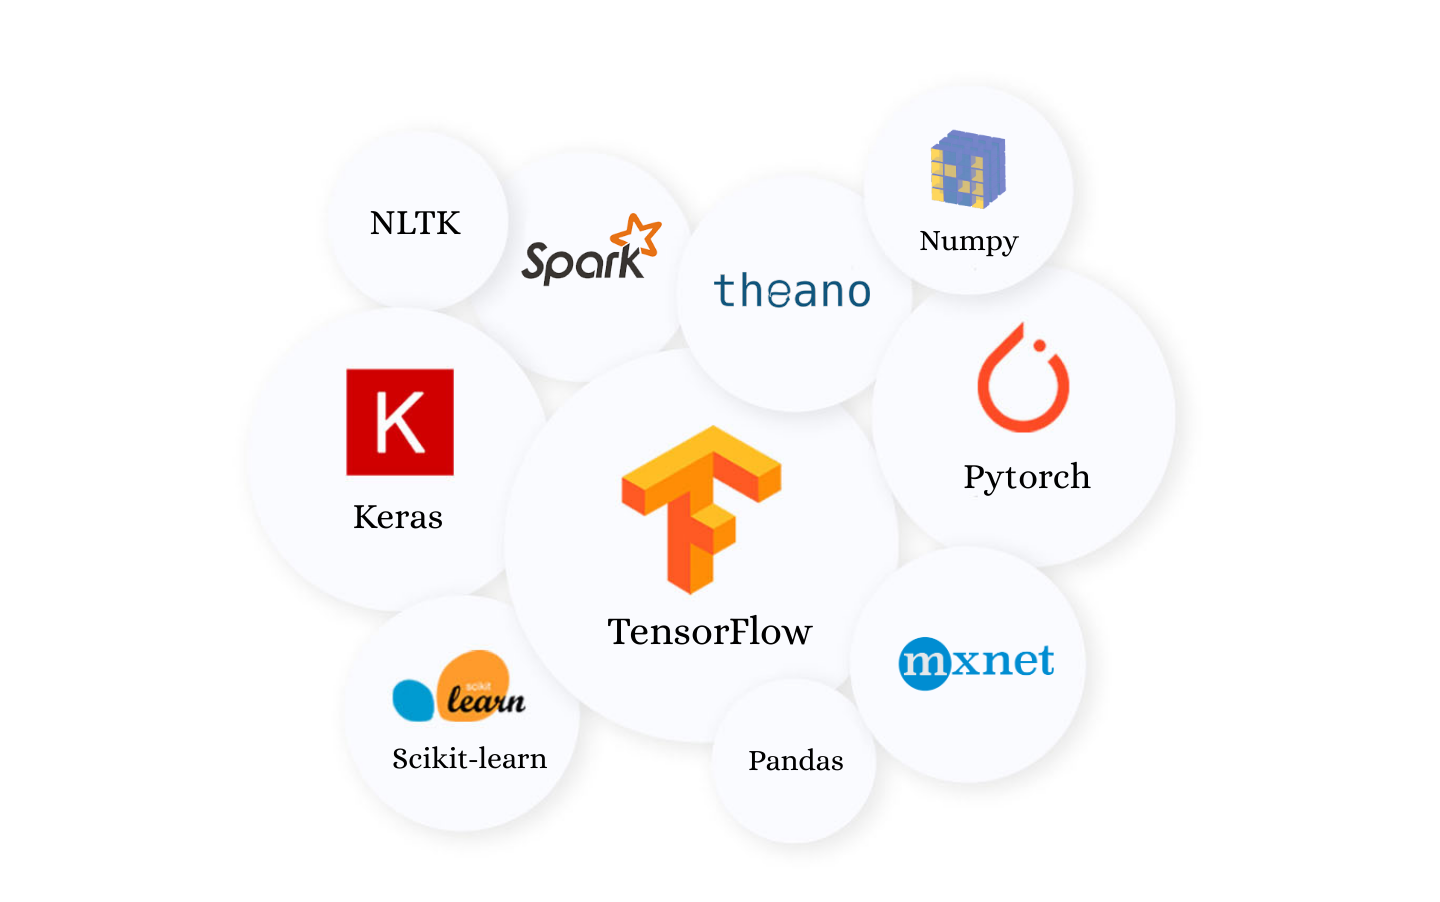
\includegraphics[width=1.1\textwidth]{images/libraries.png}
                    \caption*{{\sl Python statistics libraries}}
                \end{figure}
            \end{center}
        \end{column}
        \begin{column}{0.5\textwidth}
            \begin{itemize}
                \item Research using stastical and/or machine learning tools
                depends on increasingly complex software stacks
                \item Replicating a result becomes difficult due to 
                incomplete dependencies, platform incompatibilites $\ldots$ 
            \end{itemize}
        \end{column}
    \end{columns}
\end{frame}

\begin{frame}{Common Reproducibility Issues (2)}
    \begin{columns}
        \begin{column}{0.5\textwidth}  %%<--- here
            \begin{center}
                \begin{figure}
                    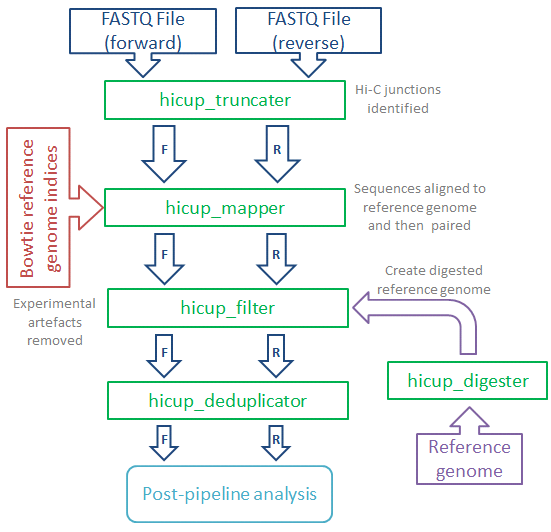
\includegraphics[width=1.1\textwidth]{images/pipeline.png}
                    \caption*{{\sl A bioinformatics data pipeline}}
                \end{figure}
            \end{center}
        \end{column}
        \begin{column}{0.5\textwidth}
            \begin{itemize}
                \item Data processing pipelines have many interdependant steps
                from the raw data to a final result 
                \item Replicating a workflow will involve difficult guesswork if these steps not properly documented 
            \end{itemize}
        \end{column}
    \end{columns}
\end{frame}

\begin{frame}{Popper}
    \begin{columns}
        \begin{column}{0.5\textwidth}  %%<--- here
            \begin{center}
                \begin{figure}
                    
\includegraphics[width=0.8\textwidth]{images/popper_logo.png}
                \end{figure}
            \end{center}
        \end{column}
        \begin{column}{0.5\textwidth}
            Popper is a container-native workflow execution engine
            which addresses these issues:
            \begin{itemize}
                \item Containerizing workflows avoids problems due to different 
                software environments
                \item Specifying steps explicitely in a Popper workflow file avoids problems due to data pipeline complexity
            \end{itemize}
        \end{column}
    \end{columns}

\end{frame}

\begin{frame}{Limitations}
    However $\ldots$
    \begin{itemize}
        \item  Popper requires fluency in DevOps tools (in particular
        container engines)
        \item Steep learning curve for users with no prior experience in these tools, who would nonetheless benefit from more reproducible workflows
    \end{itemize}
    $\rightarrow$ 
\end{frame}

\begin{frame}{Guide}

\end{frame}

\begin{frame}{Workflow Templates}

\end{frame}

\begin{frame}{Sample Workflows}
    
\end{frame}

\begin{frame}{Highlights (1)}

\end{frame}

\begin{frame}{Highlights (2)}

\end{frame}





\end{document}